\documentclass[12pt,letterpaper]{article}

\usepackage{amsmath, amsthm}
\usepackage{microtype, parskip}
\usepackage[comma,numbers,sort&compress]{natbib}
\usepackage{lineno}
\usepackage{docmute}
\usepackage{caption, subcaption, multirow, morefloats, rotating}
\usepackage{wrapfig}

\frenchspacing

\begin{document}

\section*{Introduction}

% Taxon occurrence as a function of both emergent biological traits and its environmental context?

How do species pools change over time as species are recruited or go extinct? When are ecotypes enriched or depleted? How does global and regional environmental context affect the distribution of species ecotypes (e.g. guilds) in a regional species pool?

A regional species pool is the set of species which form communities in a specific region; local communities are subsets of the regional pool. The composition of a regional species pool changes over time due to speciation, migration, extinction. Local scale processes like resource competition only affect the regional species pool if all communities are affected.

Valentine and Bambach how they presented guilds in paleobiology. Bush and Bambach presented an ecocube to describe what how marine invertebrates partition space and resources CITATION. Unique combinations represent what possible ecotypes are observable. The distribution of ecocube occupancy is then normally analyzed using ordination methods and the change in disparity over is estimated CITATION.

Fourth-corner modeling is concerned with explaining either species abundance or presence/absence as a product of species traits, environmental factors, and the interaction between these factors. In modern ecological studies, the matrix being modeled is of species occurrence at localities distributed in region. In this study, the matrix being modeled is of species occurrence in temporal bins across the Cenozoic in North America. These dimensions are all axes of the same three dimensional occurrence matrix: species by locality by time.

One of the greatest challenges with analyzing species occurrence data is the inherent incompleteness of any sample CITATION. In the modern, only presences are certain as an absence can be caused by both the species being truly absent or the species never having been sampled CITATION. For paleontological data in the context of this study, the incomplete preservation of fossil communities combined with the incomplete sampling of what fossils there are means that the true times of origination or extinction may not be observed CITATION.

\citet{Smits2015} found several systematic differences in mammal species durations associated with various species traits. Omnivorous taxa were found to have, on average, a greater duration than other dietary categories. Additionally, arboreal taxa were found to have a shorter duration than other locomotor categories. 

An unresolved question from \citet{Smits2015} is whether the greater extinction risk faced by arboreal is constant over time or if there was a change in extinction risk at the Paleogene/Neogene boundary. Specifically, the question is whether the extinction risk arboreal taxa increased in the Neogene, driving the loss of arboreal taxa and average extinction risk of arboreal taxa down. 

There are no observed massive taxonomic turnover events in the North American record, unlike the Neogene record Europe CITATION ALROY OTHERS.

% effect of climate on diversification process
The effect of climate on diversity and the diversification process has been the focus of considerable research with many analyses favoring diversification being more biologically-mediated than climate-mediated CITATION. Scale of analysis makes a big difference in interpretation of results, both temporal and geographic. For example when the mammal fossil record analyzed at small temporal and geographic scales a correlation between diversity and climate are observable CITATION CLYDE. However, when the record is analyzed at the scale of the continent and the Cenozoic there is no correlation with diversity and climate CITATION ALROY. This results, however, does not go against the idea that there may be short periods of correlation and that this correlation change or reverse direction over time; instead this result means that there is no single direction of correlation between diversity and climate.

There are many global climatic events that may have influenced the distribution of mammal ecotypes regionally, if not globally CITATION. PETM. The Mid-Miocene climactic optimum. The general cooling throughout the Cenozoic and the development of ice-caps in the Neogene. The Oligo-Miocene boundary. The transition from the Paleogene to the Neogene in North America is typically described as the ``opening-up'' of the landscape as partially forested environments were replaced by savannah and grasslands CITATION.


% events of interest
%   faunal shift at Paleogene-Neogene boundary
%     Oligo-Miocene boundary (Chattian--Aquitanian)
%     no known climatic events
%     from kind of modern to mostly modern species pool
%     (mulitple european events)
%   rise of grasses
%     janis
%     stromberg
%     (fortelius and europe)
%   other climate events? PETM, mid-miocene climatic optimum

\begin{figure}[ht]
  \centering
  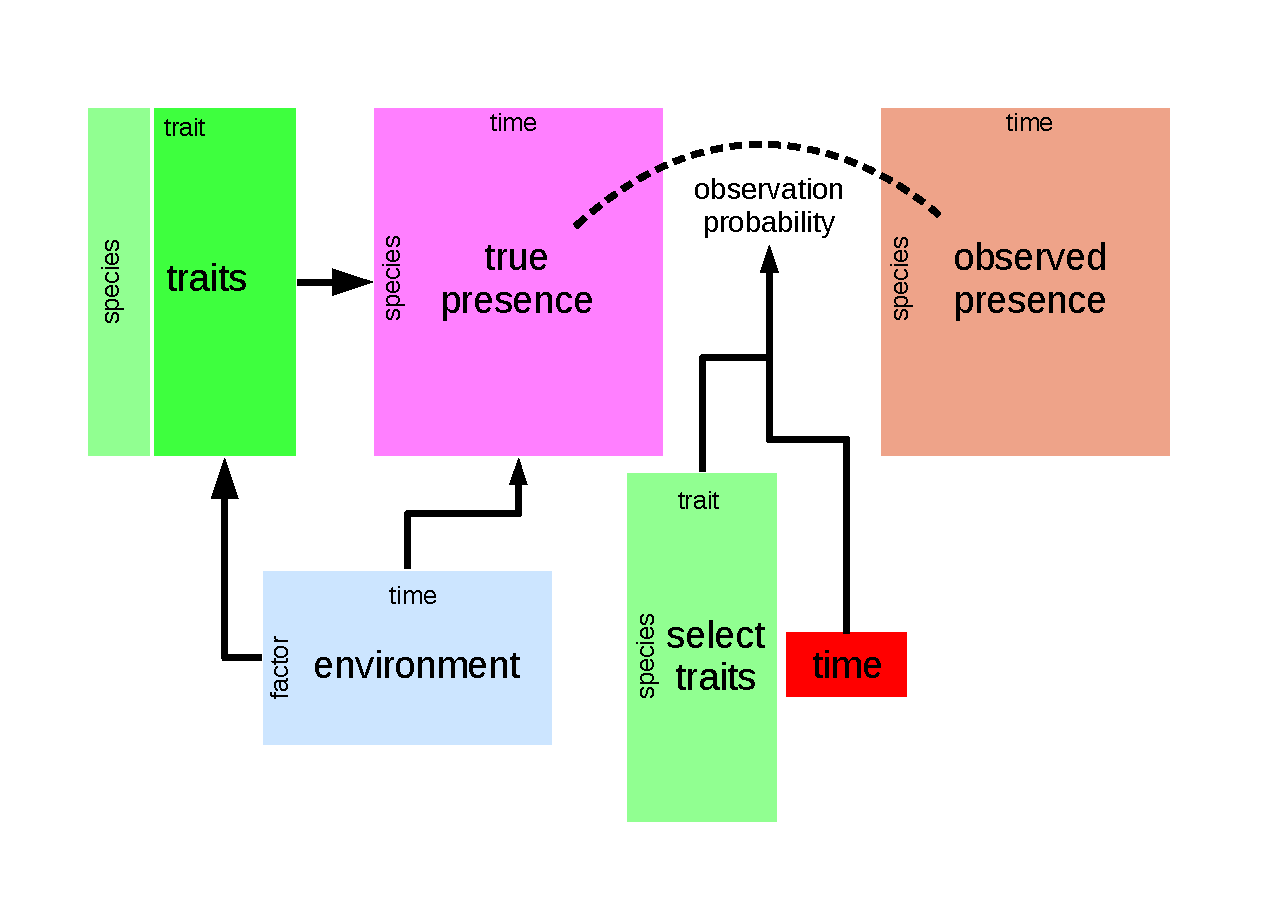
\includegraphics[width=\textwidth,height=0.8\textheight,keepaspectratio=true]{figure/paleo_fourth_corner}
  \caption{Conceptual diagram of the paleontological fourth corner problem. Figure is based on CITATION}
  \label{fig:concept_fourth_corner}
\end{figure}

% individual-level covariates
%   intercept term, varying by time
%   locomotor type/category
%       arboreal, digitigrade, plantigrade, unguligrade, fossorial, scansorial
%   dietary category
%     carnivore, herbivore, insectivore, omnivore
%   body size
%     rescale of log body mass

% group-level covariates
%   intercept
%   mean of temperatue estimate at time t
%   interquartile range of temperatue estimate at time t
%   plant community phase following Graham

% compare model assuming perfect sampling to model allowing for imperfect sampling
% imperfect sampling
%   two-state, discrete time hidden markov model with absorbing state
%     observation model for Royle and Dorazio
%     used a lot in paleobiology
%       Liow
%   a continuous-time analogue would be PyRate
%     strong assumptions about probability of observing over species duration
% issues surrounding model complexity
%   including covariates adds a lot of complexity
%   only doing approximate Bayesian inference (ADVI)
%   see methods section for longer discussion

% why consider phylogeny?
%   may or may not be an issue in community ecology/assembly/whatever the fuck
%     that's whatever
%   but i'm doing stuff over time
%     so we actually progress along the tree
%     much better change of phylogeny actually mattering
%       clade replacement in NA (carnivores, herbivores, etc)
%   so i'm just thinking of it as how it affects occurrence
%     GLMM approach is super effective for this purpose
%   note that i'm not actually modeling the diversification process
%     that's what a true J-S model (or PyRate) do
%     i'm just accounting for phylogenetic autocorrelation in species occurrence


% goals of this analysis
%   questions being addressed
%   how these questions are answered

\end{document}
